\documentclass[10pt,a4paper]{scrartcl}
\pagestyle{empty}
\usepackage{a4} % alternativ \usepackage{a4wide}
\usepackage[ngerman]{babel} % Neudeutsche Silbentrennung (mehrsprachiges Dokument)
\usepackage{parskip} % Skip indentation of first row
\usepackage{graphicx} % Graphics support
\usepackage{longtable} % Tables across several pages
\usepackage{booktabs}
\usepackage{hyperref} % Hyperlinks
\usepackage{float} % Force float position
\usepackage[automark]{scrpage2} %kopf/fusszeile
\usepackage[utf8x]{inputenc} % Unicode-Encoding
 
\linespread{1.3}

\author{Danilo Bargen, Christian Fässler, Jonas Furrer} 
\title{Zeitmanagement\\ Projekt BierIdee}

\pagestyle{scrheadings}
\ihead{SE2 Projekte} %linke Kopfzeile
\ohead{BierIdee} %rechte Kopfzeile

\begin{document}

\begin{titlepage}
	\maketitle
	\vspace{120mm}
	\thispagestyle{empty} % Don't start page numbers on this page
\end{titlepage}

\tableofcontents
\newpage

\section*{Änderungshistorie}
\begin{tabular}{p{0.1\textwidth}p{0.15\textwidth}p{0.55\textwidth}p{0.1\textwidth}}
\toprule
\textbf{Version} & \textbf{Datum} & \textbf{Änderung} & \textbf{Person} \\  
\midrule
v1.0 & 31.05.2012 & Dokument erstellt & dbargen \\  
\bottomrule
\end{tabular} 
\newpage

\section{Commit-Aktivität}

Auf Github kann man Statistiken über die Commit-Aktivität generieren. Nachfolgend die
"`Punchcard"'-Diagramme für das Front- und das Backend. Je grösser der schwarze Punkt, desto mehr
Commits wurden in dieser Zeit erstellt.

\begin{figure}[H]
	\begin{center}
		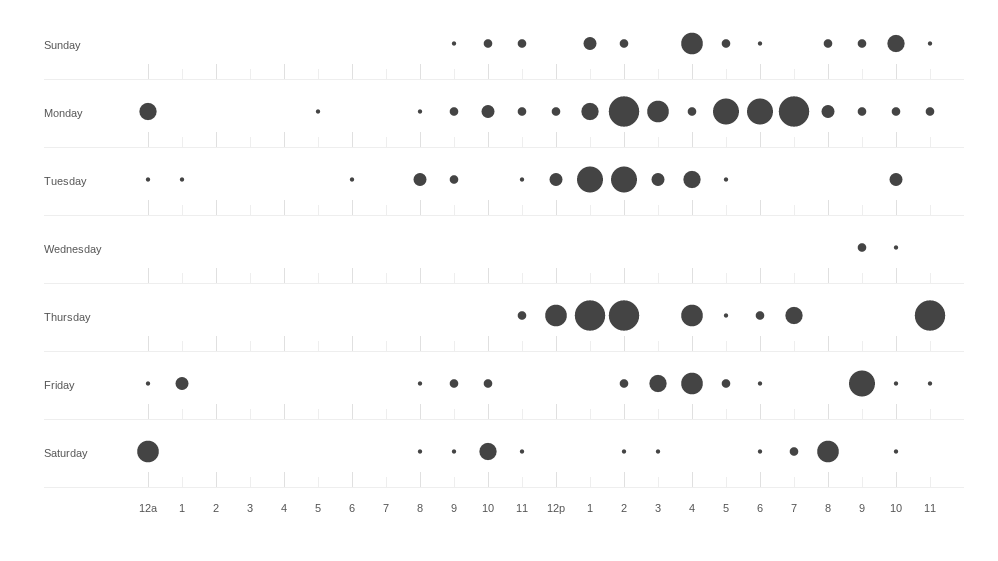
\includegraphics[width=\textwidth]{img/punchcard_front.png}
	\end{center}
	\caption{Commit-Aktivität Frontend}
\end{figure}

\begin{figure}[H]
	\begin{center}
		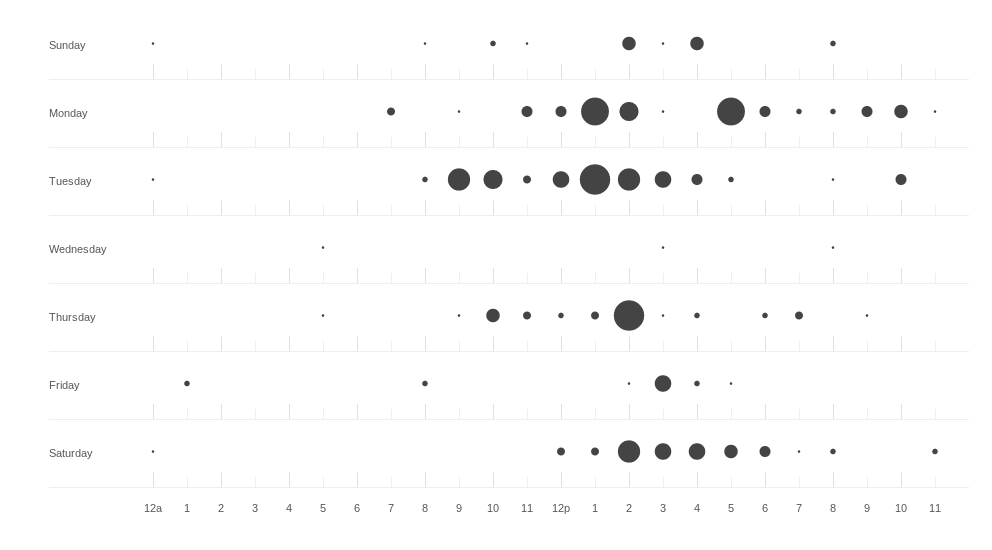
\includegraphics[width=\textwidth]{img/punchcard_back.png}
	\end{center}
	\caption{Commit-Aktivität Backend}
\end{figure}

\newpage
Da wir auch für die Dokumentation ein Repository eingerichtet haben, kann man auch dort das Diagramm
betrachten:

\begin{figure}[H]
	\begin{center}
		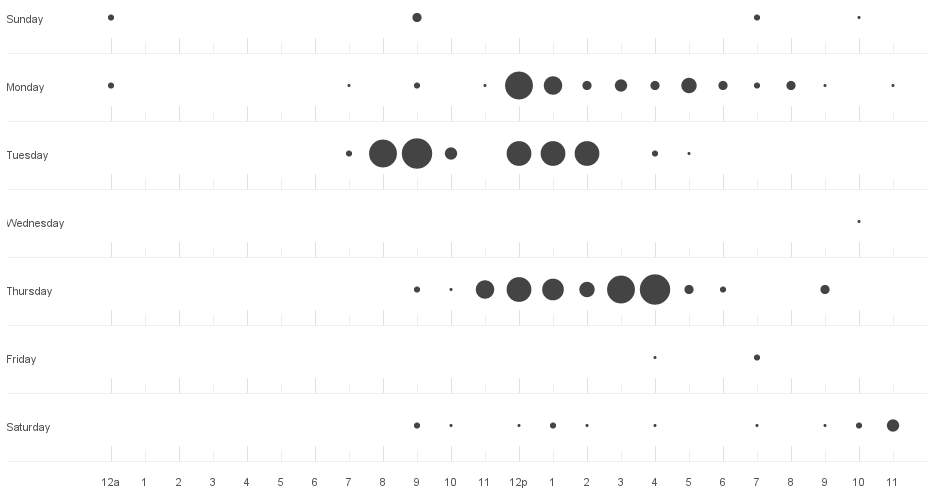
\includegraphics[width=\textwidth]{img/punchcard_docs.png}
	\end{center}
	\caption{Commit-Aktivität Dokumentation}
\end{figure}

Hier sieht man schön, dass praktisch nur an den Tagen gearbeitet wurde, an denen wir an der HSR
waren, während sich die (eher interessante) Programmierarbeit über die gesamte Woche erstreckte.


\newpage
\section{Zeitaufwand Diagramme}

Nachfolgend zwei Diagramme mit Auswertungen zu unseren Zeitaufwänden und jeweils einem kurzen Kommentar.

\subsection{Arbeitsaufwand pro Semesterwoche}

\begin{figure}[H]
	\begin{center}
		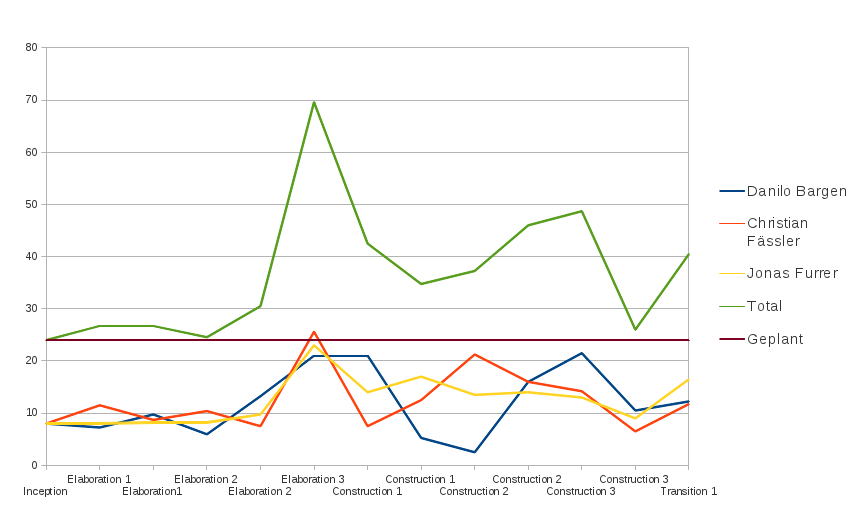
\includegraphics[width=\textwidth]{img/time_diagram.png}
	\end{center}
	\caption{Arbeitsaufwand während dem Semester}
\end{figure}

Der Peak während der Elaboration 3 Phase kommt daher, dass wir da den Architekturprototypen
fertigstellen mussten, was wegen der Datenbank-Umstellung viel Zeit gekostet hat.

\subsection{Arbeitsaufwand pro Projektphase}

\begin{figure}[H]
	\begin{center}
		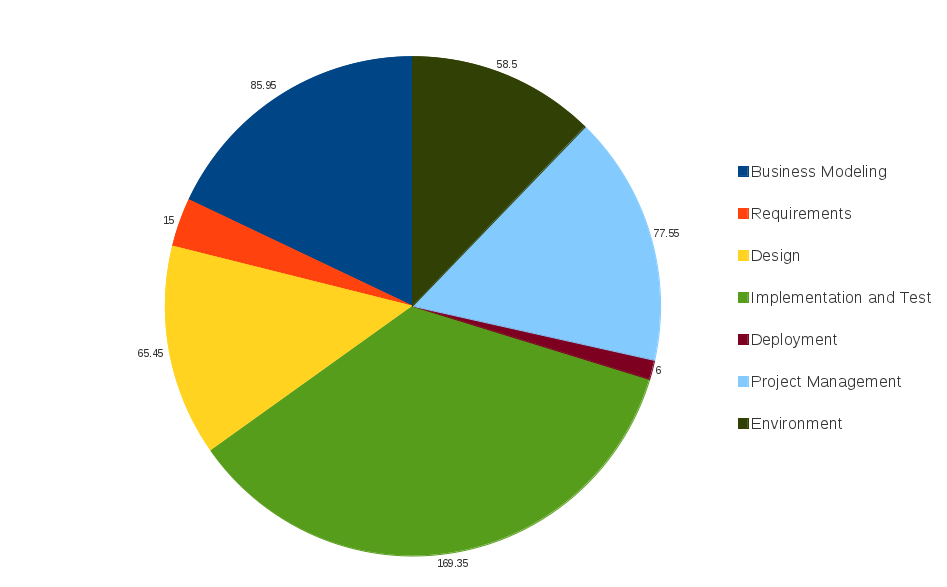
\includegraphics[width=\textwidth]{img/timelog_tracker.png}
	\end{center}
	\caption{Verteilung Aufwand auf Projektphasen}
\end{figure}

Der grösste Teil der Arbeitszeit fällt auf die "`Implementation and Test"` Phase. Die Phasen
"'Project Management"` "'Design"` "'Business Modeling"` und "'Environment"` sind alle etwa gleich
stark vertreten. Die "'Requirements"`-Definition sowie das "'Deployment"` sind in diesem Projekt
sehr schwach vertreten.




\end{document}
